\documentclass{ximera}

\newcommand{\RR}{\mathbb R}
\renewcommand{\d}{\,d}
\newcommand{\dd}[2][]{\frac{d #1}{d #2}}
\renewcommand{\l}{\ell}
\newcommand{\ddx}{\frac{d}{dx}}
\newcommand{\dfn}{\textbf}
\newcommand{\eval}[1]{\bigg[ #1 \bigg]}


\author{Jim Fowler}
\license{Creative Commons 4.0 By-SA}

\begin{document}

\begin{exercise}
  Consider the vector $\vec{v}$.
  \begin{image}
    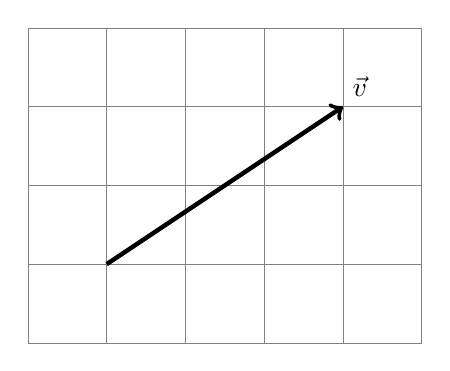
\begin{tikzpicture}
      \draw[step=1cm,gray,very thin] (-1,-1) grid (4,3);
      \draw[->,ultra thick] (0,0) -- (3,2);
      \node[anchor=south west] at (3,2) {$\vec{v}$};            
    \end{tikzpicture}
  \end{image}
  What are the coordinates of $\vec{v}$?
  \[
    \vec{v} = \vector{\answer{3},\answer{2}}.
  \]
  
\end{exercise}

\end{document}

%%% Local Variables:
%%% mode: latex
%%% TeX-master: t
%%% End:
